\chapter {DASAR TEORI}

Pada bab ini, akan dijelaskan dasar teori yang digunakan sebagai landasaan pengerjaan Tugas Akhir ini.

\section{Deskripsi Permasalahan}
Permasalahan yang dibahas pada Tugas Akhir ini adalah perhitungan untuk mencari nilai $x$ yang didefinisikan oleh persamaan \eqref{eq:perimeter-polygon}.
\begin{equation}
    \label{eq:perimeter-polygon}
    x=\sum_{i=0}^{n-1} \text{RCH}_i
\end{equation}
$\text{RCH}_i$ pada persamaan \eqref{eq:perimeter-polygon} menyatakan sisi polygon dari RCH yang merupakan \textit{relative convex hull} yang didapatkan dari sekumpulan titik yang dibatasi di dalam polygon sederhana\cite{isun1}. Permasalahan pada tugas akhir ini adalah mencari \textit{relative convex hull} dari sekumpulan titik yang dibatasi oleh polygon sederhana. Gambar \ref{fig:ilustrasi-contoh-kasus-tanpa-solusi} dan \ref{fig:ilustrasi-contoh-kasus} merupakan contoh dari permasalahan ISUN1.
\begin{figure}[!h]
	\Centering
	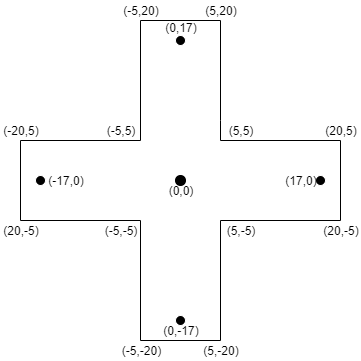
\includegraphics [width=0.5\columnwidth]{bab2/img/contoh-kasus-tanpa-solusi}
	\caption {Ilustrasi Contoh Kasus Tanpa Solusi}
	\label {fig:ilustrasi-contoh-kasus-tanpa-solusi}
\end{figure}
\begin{figure}[!h]
	\Centering
	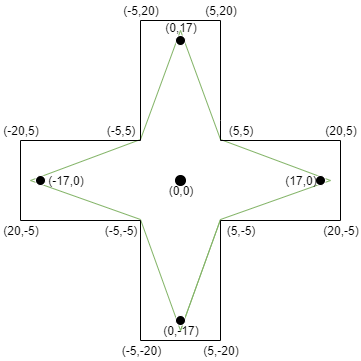
\includegraphics [width=0.5\columnwidth]{bab2/img/contoh-kasus}
	\caption {Ilustrasi Contoh Kasus}
	\label {fig:ilustrasi-contoh-kasus}
\end{figure}

\section{Convex Polygon}
\textit{Convex polygon} merupakan sebuah polygon sederhana yang memiliki sudut maksimal 180 derajat pada tiap edgenya. \textit{Convex polygon} memiliki beberapa properti, yaitu:
\begin{enumerate}
    \item Sebuah garis lurus yang di gambar melewati sebuah \textit{convex} polygon akan berpotongan maksimal 2 kali. Ilustrasi dapat dilihat pada gambar \ref{fig:ilustrasi-properti-convex-polygon-1}.
    \item Jika dua titik sembarang diambil dan ditarik garis antara keduanya, tidak ada bagian dari garis yang berada di luar polygon. Ilustrasi dapat dilihat pada gambar \ref{fig:ilustrasi-properti-convex-polygon-2}.
\end{enumerate}
\begin{figure}[!h]
    \Centering
    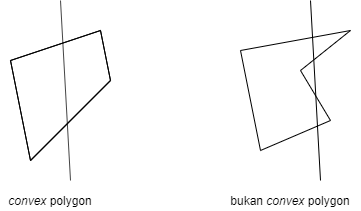
\includegraphics[width=0.5\columnwidth]{bab2/img/ilustrasi-properti-convex-polygon-1}
    \caption{Ilustrasi Properti Convex Polygon 1}
    \label{fig:ilustrasi-properti-convex-polygon-1}
\end{figure}
\begin{figure}[!h]
    \Centering
    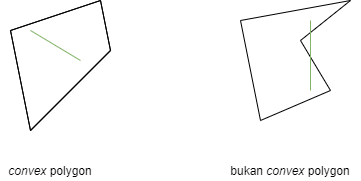
\includegraphics[width=0.5\columnwidth]{bab2/img/ilustrasi-properti-convex-polygon-2}
    \caption{Ilustrasi Properti Convex Polygon 2}
    \label{fig:ilustrasi-properti-convex-polygon-2}
\end{figure}

\subsection{Relative Convex Polygon}
\textit{Relative convex polygon} merupakan penurunan dari \textit{convex polygon} tetapi ada beberapa sisi dari polygon tersebut berbentuk \textit{convace} atau cekung kedalam dikarenakan adanya batasan dari luar seperti polygon atau segmen garis lainnya. Ilustrasi \textit{relative convex polygon} dapat dilihat pada gambar \ref{fig:ilustrasi-relative-convex-polygon}.
\begin{figure}[!h]
    \Centering
    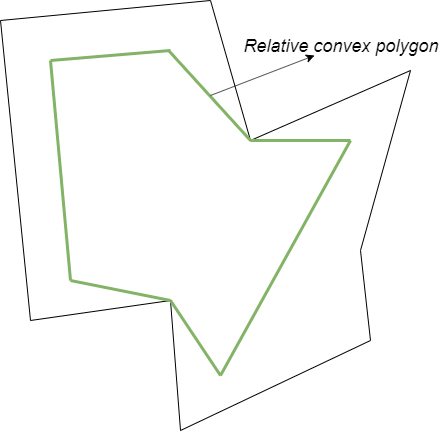
\includegraphics[width=0.5\columnwidth]{bab2/img/ilustrasi-relative-convex-polygon}
    \caption{Ilustrasi Relative Convex Polygon}
    \label{fig:ilustrasi-relative-convex-polygon}
\end{figure}
\section{Strategi Penyelesaian Permasalahan}
Pada subbab ini akan dipaparkan mengenai strategi penyelesaian masalah klasik pada daring SPOJ dengan kode ISUN1 menggunakan algoritma reduksi polygon. Secara singkat, strategi penyelesaian masalah dari ISUN1 menggunakan algoritma reduksi polygon menjadi 2 bagian besar, yaitu :
\begin{enumerate}
    \item Pemrosesan titik pembentuk polygon yang membentuk \textit{Convex}.
    \item \textit{Convex Hull} dari titik yang berada didalam polygon.
\end{enumerate}
Sebagai contoh, pada subbab ini akan menggunakan $P$ sebagai polygon luar yang mempunyai $n$ vertex, dimana $P = \left \langle p_1, p_2, ..., p_n \right \rangle$ yang mempunyai titik sebanyak $m$ ($S = \left \langle s_1, s_2, ..., s_m \right \rangle$), dan $D(A)$ merupakan sebuah deque (\textit{doubly-ended queue}) yang menampung vertex dari polygon $P$. Reduksi polygon didasari dari algoritma \textit{Melkman convex hull} dengan sedikit modifikasi. Modifikasi yang dilakukan adalah ketika 3 buah titik pembentuk polygon yang konsekutif membuat \textit{convex} maka titik tengah dari ketiga titik tersebut dibuang, dan jika \textit{concave} maka titik tengahnya tetap disimpan. Pada saat sebuah titik dibuang, maka luas dari polygon akan tereduksi. Langkah-langkah reduksi dilakukan dengan mengulangi 2 langkah yang akan dijelaskan pada subbab \ref{sec:pemrosesan-titik-pembentuk-polygon-yang-membentuk-convex} dan \ref{sec:convex-hull-dari-titik-yang-berada-di-dalam-polygon}.


\subsection{Pemrosesan Titik Pembentuk Polygon yang Membentuk Convex}
\label{sec:pemrosesan-titik-pembentuk-polygon-yang-membentuk-convex}
Pemrosesan titik pembentuk polygon dapat dilakukan dengan cara melakukan \textit{traversing} terhadap semua vertex pembentuk polygon. Untuk setiap vertex $p_i$ yang di periksa, hitung orientasi(secara berlawanan jarum jam) titik $p_i$ dengan $p_{i-1}$ dan $ p_{i+1}$. Jika orientasinya membentuk \textit{convex}, maka titik $p_i$ akan dibuang.
\par Sebelum membuang titik $p_i$, kita akan membuat sebuah segitiga $ABC$ dimana $A=p_i$, $B=p_{i-1}$, dan $C=p_{i+1}$ karena triangulation of polygon(Teorema \ref{theo:triangulation-of-polygon}).
\begin{theo}[Triangulation of Polygon]
    \label{theo:triangulation-of-polygon}
	Semua polygon dapat di buat dari beberapa segitiga.
\end{theo}
Kemudian cari $T(ABC)$ dimana $T(ABC)$ merupakan semua titik $S$ yang berada di dalam segitiga $ABC$ dengan menggunakan algoritma \textit{Point Inside Polygon} (dapat dilihat pada subbab \ref{sec:point-inside-polygon}). Pencarian titik yang berada di dalam segitiga $ABC$ berguna untuk mencari pengganti vertex $p_i$ sebagai pembentuk polygon luarnya.

\subsection{Convex Hull dari Titik yang Berada di Dalam Polygon}
\label{sec:convex-hull-dari-titik-yang-berada-di-dalam-polygon}
Melanjutkan dari subbab \ref{sec:pemrosesan-titik-pembentuk-polygon-yang-membentuk-convex}, ketika sudah mendapatkan $T(ABC)$, lakukan pencarian \textit{Convex Hull} dari titik - titik tersebut menggunakan algoritma \textit{monotone chain} (dapat dilihat pada subbab \ref{sec:algoritma-monotone-chain}). Kemudian sisipkan semua titik yang membentuk \textit{Convex Hull} diantara vertex $p_{i-1}$, $p_{i+1}$ untuk me-rekonstruksi polygon luar yang sudah di reduksi.

\section{Convex Hull}
\label{sec:convex-hull}
\textit{Convex Hull} dari sekumpulan titik $S$ adalah sebuah set dari semua kombinasi \textit{convex} dari titik - titik tersebut. Setiap titik $s_i$ pada $S$ diberikan sebuah koefisien $a_i$ dimana $a_i$ merupakan bialangan non negatif dan jika semua $a_i$ dijumlahkan hasilnya satu. Dan koefisien ini digunakan untuk menghitung berat rata - rata untuk setiap titik. Untuk setiap koefisien yang dipilih akan dikombinasikan dan menghasilkan \textit{convex hull}. Set \textit{convex hull} ini dapat di ekspresikan dengan formula \eqref{eq:convex-hull} dan ilustrasi \textit{convex hull} ada pada gambar \ref{fig:ilustrasi-convex-hull}.

\begin{equation}
    \label{eq:convex-hull}
    Conv(S)=\left\{ \sum_{i=1}^{|S|}{a_is_i} \big | (\forall{i}:a_i \ge 0 \wedge \sum_{i=1}^{|S|}{a_i=1} ) \right\}
\end{equation}
\begin{figure}[!h]
	\Centering
	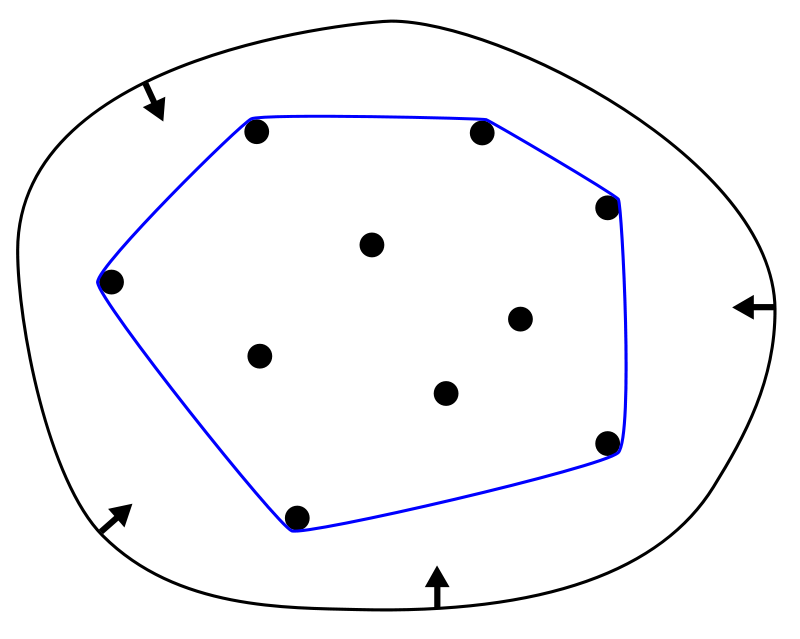
\includegraphics [width=0.5\columnwidth]{bab2/img/ilustrasi-convex-hull}
	\caption {Ilustrasi Convex Cull}
	\label {fig:ilustrasi-convex-hull}
\end{figure}


\subsection{Relative Convex Hull}
\textit{Relative convex hull} merupakan penurunan dari \textit{convex hull}. \textit{Relative convex hull} merupakan \textit{convex hull} yang mempunyai \textit{cavity} (cekungan kedalam) yang diakibatkan atau relatif terhadap sesuatu yang membatasi \textit{convex hull} tersebut. ilustrasi \textit{relative convex hull} dapat dilihat pada gambar \ref{fig:ilustrasi-relative-convex-hull}.

\begin{figure}[!h]
	\Centering
	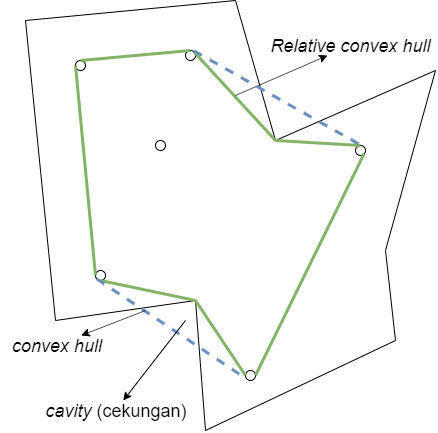
\includegraphics [width=0.5\columnwidth]{bab2/img/ilustrasi-relative-convex-hull}
	\caption {Ilustrasi Relative Convex Hull}
	\label {fig:ilustrasi-relative-convex-hull}
\end{figure}
\par Penentuan untuk mengetahui sebuah polygon merupakan \textit{convex} atau \textit{concave} dapat menggunakan orientasi. Apabila orientasi dari tiga titik yang berurutan adalah positif berlawanan jarum jam maka tiga titik tersebut adalah \textit{convex}. Sebaliknya apabila negatif maka tiga titik tersebut adalah \textit{concave}. Untuk mencari orientasi antara tiga titik dapat digunakan persamaan \ref{eq:orientasi}.
\begin{equation}
    \begin{aligned}
    \label{eq:orientasi}
        \vec{u}&=(B_x-A_x)x +(B_y-A_y)y\\
        \vec{v}&=(C_x-A_x)x +(C_y-A_y)y\\
    \end{aligned}
\end{equation}
$$ Orientasi = u_x*v_y - u_y*v_x $$
\subsection{Algoritma Convex Hull}
Ada beberapa algoritma yang dapat digunakan untuk mencari sebuah \textit{convex hull}, untuk melihat perbandingan dari beberapa algoritma dapat dilihat pada tabel \ref{tab:tabel-algoritma-convex-hull}.
\begin{table}[]
    \Centering
    \newcolumntype{P}[1]{>{\centering\arraybackslash}p{#1}}
    \caption{Tabel Perbandingan Algoritma Convex Hull}
    \label{tab:tabel-algoritma-convex-hull}
    \begin{tabular}{|P{2cm}|P{2cm}|P{2cm}|P{1.5cm}|P{2cm}|}
        \hline
    Algoritma Convex Hull & Implementasi & Kompleksitas & Kode Sumber     & Jenis Input \\ \hline
    Jarvis's Algorithm    & Mudah                  & $\mathcal{O}(n^2)$         & Singkat         & Kumpulan Titik\\ \hline
    Graham's Scan         & Sedikit Mudah          & $\mathcal{O}(n\log(n))$  & Singkat         & Kumpulan Titik  \\ \hline
    Quick Hull            & Kompleks               & $\mathcal{O}(n\log(n))$  & Panjang         & Kumpulan Titik  \\ \hline
    Monotone Chain        & Mudah                  & $\mathcal{O}(n\log(n))$  & Singkat         & Kumpulan Titik  \\ \hline
    Melkman's Algorithm   & Mudah                  & $\mathcal{O}(n)$           & Singkat         & polygon Sederhana \\ \hline    
    \end{tabular}
\end{table}
Berdasarkan tabel \ref{tab:tabel-algoritma-convex-hull}, penulis memilih 2 algoritma yang akan digunakan pada buku ini.
\subsubsection{Algoritma Melkman Convex Hull}
\label{sec:algoritma-melkman-convex-hull}
Algoritma melkman \textit{convex hull} merupakan algoritma untuk menghitung rantai polygonal ataupun polygon sederhana dengan waktu linear $\mathcal{O}(n)$\cite{melkman_algorithm}. Asumsikan sebuah polygon sederhana $P$, dengan vertex $p_i$ dan edge $p_i p_{i+1}$. Algoritma ini menggunakan deque, $D = \left \langle d_1, d_2, ..., d_n \right \rangle$, untuk mereprentasikan \CH, $Q_i = CH(P_i)$, dimana $P_i = (p_0, p_1, ..., p_i)$. Deque mempunyai fungsi \textit{push} dan \textit{pop} dari atas/depan dan \textit{insert} dan \textit{remove} dari bawah/belakang. Secara spesifiknya yang dilakukan \textit{push} $v$ ke deque melakukan $(l \leftarrow l+1; d_t \leftarrow v)$, untuk \textit{pop} $d_t$ dari deque melakukan $(t \leftarrow t-1)$, untuk insert $v$ ke deque melakukan $(b \leftarrow b-1; d_b \leftarrow v)$, dan \textit{remove} $d_b$ dari deque melakukan $(b \leftarrow b+1)$.
\par Algoritma ini menggunakan konvensi dimana vertexnya berurutan secara berlawanan jarum jam di sekitar \CH $Q$.
\par Setiap $d_t$ dan $d_b$ mengacu kepada vertex yang sama pada rantai polygon $C$, dan vertex ini akan selalu menjadi vertex yang kita tambahkan terakhir pada \CH. Pseudocode Melkman Convex Hull dapat dilihat pada pseudocode \ref{psdo:Melkman-Convex-Hull}.
\begin{figure}[!h]
	\Centering
	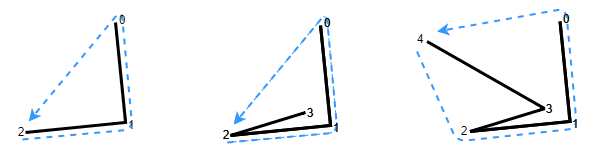
\includegraphics [width=\columnwidth]{bab2/img/ilustrasi-algoritma-melkman}
	\caption {Ilustrasi Algoritma Melkman}
	\label {fig:ilustrasi-algoritma-melkman}
\end{figure}
\begin{algorithm}
	\caption{Melkman Convex Hull}
	\label{psdo:Melkman-Convex-Hull}
	\begin{algorithmic}[1]
		\Require $P$
		\Ensure $Q$
        \State Inisialisasi: $D$
        \If{\fakesc{Left}($p_0, p_1, p_2$)}
            \State$D \leftarrow \left \langle p_2, p_0, p_1, p_2 \right \rangle$
        \Else
            \State $D \leftarrow \left \langle p_2, p_1, p_0, p_2 \right \rangle$
        \EndIf
        \State $i=3$
        \While{$i<n$}
            \While{ \fakesc{Left}($d_{t-1}, d_t, p_i$) dan \fakesc{Left}($d_b, d_{b+1}, p_i$))} 
                \State $i \leftarrow i+1$
            \EndWhile
            \While{!\fakesc{Left}($d_{t-1}, d_t, p_i$)}
                \State \textit{pop} $d_t$
            \EndWhile
            \State \textit{push} $p_i$
            \While{!\fakesc{Left}($p_i,d_{b}, d_{b+1}$)}
                \State \textit{remove} $d_b$
            \EndWhile
            \State \textit{insert} $p_i$
            \State $i \leftarrow i+1$
        \EndWhile
	\end{algorithmic}
\end{algorithm}

\subsubsection{Algoritma Monotone Chain}
\label{sec:algoritma-monotone-chain}
Algoritma \MC merupakan proses pembentukan \CH dari sekumpulan titik dengan kompleksitas $\mathcal{O}(n$ log$(n))$\cite{monotone_chain_algorithm}. Asumsikan sekumpulan titik $S$ sejumlah $n$ ,$S = \left \langle s_1, s_2, ..., s_n\right \rangle$ algoritma ini menggunakan list untuk membentuk sebuah rantai (\textit{monotone chain}), dimana list $L(S)$ menampung semua titik yang ada di $S$ yang terurut berdasarkan nilai koordinatnya terhadap sumbu $x$. algoritma ini memeriksa setiap 3 vertex yang berurutan, jika 3 vertex tersebut membuat \textit{convex} makan ketiga vertex tersebut disimpan, dan sebaliknya jika ketiga vertex tersebut membuat \textit{concave} maka vertex ke 2 akan dibuang dari vertex penyusun \textit{convex hull}. lalu lakukan hal yang sama dengan membalikan urutan pada $L$ untuk mendapatkan \textit{lower hull}. Pseudocode algoritma \textit{Monotone Chain} dapat dilihat pada pseudocode \ref{psdo:Monotone-Chain-Algorithm}.

\begin{figure}[!h]
	\Centering
	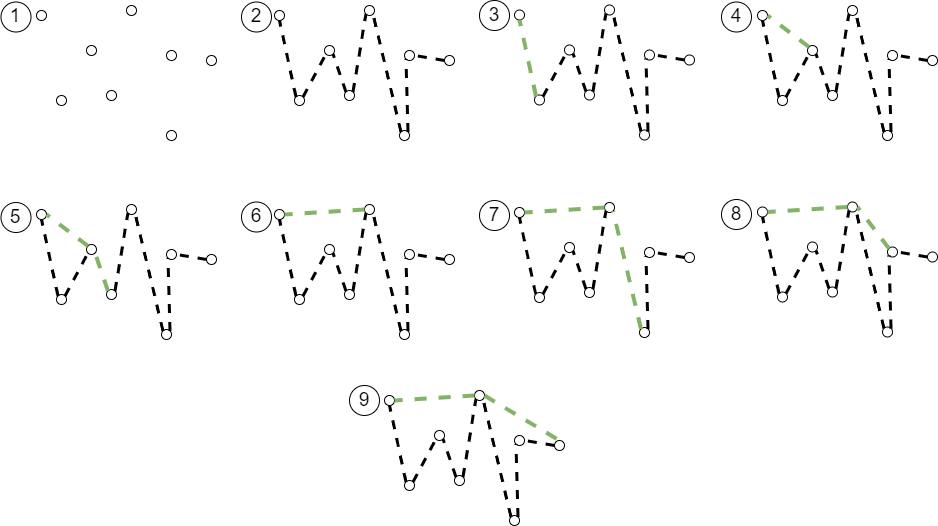
\includegraphics [width=\columnwidth]{bab2/img/ilustrasi-algoritma-monotone-chain}
	\caption {Ilustrasi Algoritma Monotone Chain}
	\label {fig:ilustrasi-algoritma-monotone-chain}
\end{figure}

\begin{algorithm}
	\caption{Monotone Chain Algorithm}
	\label{psdo:Monotone-Chain-Algorithm}
	\begin{algorithmic}[1]
		\Require $S$
		\Ensure $CH(S)$
        \State Inisialisasi: $L$
        \State Sort $S$
        \State $L \leftarrow S$
        \State Inisialisasi $CH(S)$
        \For{$i=0;i<2;i++$}
            \For{$j=0;j<Size(L);j++$}
                \While{$Size (CH)\ge2$ and $right(CH[Size(CH)-1],CH[Size(CH)-2],S[j])$}
                    \State Delete $CH$ last element
                \EndWhile
                \State push $pt$ to $CH$
            \EndFor
            \State reverse $L$
        \EndFor
	\end{algorithmic}
\end{algorithm}
\section{Point Inside Polygon}
\label{sec:point-inside-polygon}
\textit{Point inside polygon} merupakan algoritma untuk menentukan apakah suatu polygon berada di dalam sebuah polygon atau tidak \cite{point_inside_polygon}. Ide utama dari algoritma ini adalah dengan cara menarik garis sejajar dengan sumbu $x$ dimana garis tersebut berujung pada titik yang ingin dicari lokasinya kemudian hitung ada berapa \textit{edge} dari polygon yang berpotongan dengan garis tersebut. Jika jumlah \textit{edge} polygon yang berpotongan adalah ganjil, maka titik tersebut berada dalam polygon, dan sebaliknya, jika jumlahnya genap maka titik tersebut berada di luar polygon.

\begin{figure}[!h]
	\Centering
	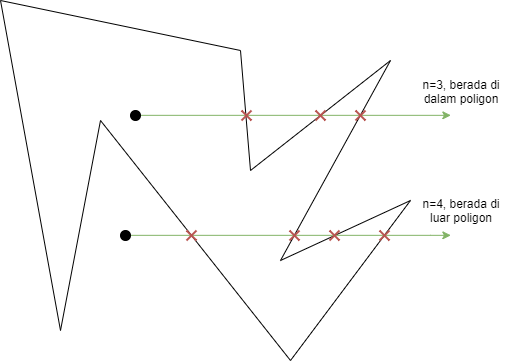
\includegraphics [width=0.5\columnwidth]{bab2/img/ilustrasi-algoritma-point-inside-polygon}
	\caption {Ilustrasi Algoritma Point Inside Polygon}
	\label {fig:ilustrasi-algoritma-point-inside-polygon}
\end{figure}
